\documentclass[11pt,a4paper]{article}
\usepackage{amsmath,amssymb,amsthm}
\usepackage{graphicx}
\usepackage{hyperref}
\usepackage{microtype}
\usepackage{geometry}
\geometry{margin=2.5cm}

\newtheorem{hypothesis}{Hypothesis}[section]
\newtheorem{proposition}{Proposition}[section]
\newtheorem{definition}{Definition}[section]
\newtheorem{remark}{Remark}[section]

\title{Exact Weil-Block Projective Capacity on Heisenberg Graphs:\\
Resolving the Final Obstruction to $\delta$ Extraction}
\author{J\'er\^ome Beau\\
\small Independent Researcher\\
\small \href{mailto:jerome.beau@cosmochrony.org}{jerome.beau@cosmochrony.org}}
\date{March 2026}

\begin{document}

  \maketitle

  \begin{abstract}
    The O-series has progressively identified and resolved a sequence of obstructions
preventing reliable extraction of the capacity exponent~$\delta$ from discrete Heisenberg
geometries: a geometric obstruction (O8--O9), an algorithmic obstruction (O10), and a
residual representation-level ambiguity at the proxy stage (O11).
O11 introduced a bidimensional Fourier-character proxy for the Weil-block decomposition,
obtaining a stable estimate $\hat{\delta}_{\mathrm{cap}}\approx 3.4$ at $q=307$ while
coarse-graining away the central coordinate~$\gamma$.
The present paper closes this observable gap by implementing the exact Weil projection,
and derives, in closed form, the intrinsic asymptotic exponent of the resulting
observable~$\Sigma_n^{(c)}$.
For each generic Weil block~$H_c$ ($c\neq 0$), we maintain a $q\times q$ span tracker
operating directly in the irreducible representation of $\mathrm{Heis}_3(\mathbb{Z}/q\mathbb{Z})$,
at primes $q\in\{29,53,61\}$, and extract finite-$q$ fitted slopes
$\hat{\delta}_{\mathrm{exact}}\in\{4.37,4.28,4.80\}$ (all $R^2>0.98$), independently
reproduced by pure combinatorial set arithmetic.
We show that $\Sigma_n^{(c)}$ admits an exact closed form depending on the block~$c$ only
through a projective pair $(\alpha,\beta)$, and is consequently, by algebraic identity and
not merely as an empirical regularity, exactly independent of the translational
coordinate~$a$ and of the central coordinate~$\gamma$: no coherence or metaplectic-phase
mechanism can affect it.
Using this closed form, we prove that the finite-$q$ fitted slopes above are crossover
statistics of the block saturation-depth distribution, not estimates of an intrinsic
asymptotic exponent, and derive the latter exactly: in the double limit $q\to\infty$,
$n\to\infty$, $n=o(\sqrt{q})$, under uniform sampling of generic blocks,
$\Sigma_n^{(c)}\sim\mathrm{const}\cdot n^{-3}$ holds block-by-block with probability
$1-O(n/q)$, from Heisenberg shell growth alone.
No constraint on the cascade exponent~$\beta^*$ is drawn from these results: substituting
either the finite-$q$ slopes or the unfolded exponent into the O3--O7 structural relation
$\beta^*=1/(\delta+\tfrac12)$ presupposes an answer, not settled here, to which of these
regimes that relation's derivation takes as input.

  \end{abstract}

  \paragraph{Keywords.}
    projective capacity, Heisenberg graphs, Weil representation, exact block projection,
    capacity exponent, metaplectic phase, polynomial growth, spectral admissibility, cascade exponent.

    \clearpage
    \tableofcontents

  \section{Introduction}

  \subsection{The O-series chain: from obstruction to extraction}

    The capacity exponent~$\delta$ encodes the sub-linear energy-rank relation predicted
    by the Cosmochrony spectral framework~\cite{Cosmochrony}.
    Its extraction from discrete graph models has been the central objective of the O-series,
    which has successively resolved a chain of obstructions.

    \textbf{O8}~\cite{Beau2026a12} established the three-step permutation-path fingerprint on
    Lubotzky--Phillips--Sarnak (LPS) expander graphs and encountered a geometric obstruction:
    the exponential shell growth $|S_n|\sim p^n$ compresses the entire pre-saturation window
    into $O(\log q)$ BFS steps, preventing stable log-log slope estimation.

    \textbf{O9}~\cite{Beau2026a13} resolved this geometric obstruction by replacing LPS graphs
    with Cayley graphs of the discrete Heisenberg group $\mathrm{Heis}_3(\mathbb{Z}/q\mathbb{Z})$,
    whose polynomial ball growth $|B_n|\sim n^4$ (Bass--Guivarc'h theorem, homogeneous
    dimension $D_{\mathrm{hom}}=4$) restores an exploitable BFS window.

    \textbf{O10}~\cite{Beau2026a14} performed the first large-$q$ computation ($q=101$,
    $|G_q|=1{,}030{,}301$) and identified an algorithmic obstruction:
    the dense TensorSketch fingerprint is structurally mismatched to the problem,
    requiring sketch dimension $D\gg q^4$ to resolve the pre-saturation window,
    which is computationally impractical.
    O10 concluded that the remaining obstruction is representational, not geometric,
    and identified the Weil-block decomposition as the correct instrument.

    \textbf{O11}~\cite{Beau2026a15} addressed this by introducing a bidimensional
    Fourier-character proxy for the Weil-block decomposition.
    The proxy acts on the abelianised coordinates $(a,b)$ of $G_q$, yielding a proxy
    ambient dimension~$q^2$ that delays saturation to the correct scale.
    All three measurability conditions (B1)--(B3) were satisfied at all tested primes
    $q\in\{101,151,211,307\}$, and a stable decay exponent
    $\hat{\delta}_{\mathrm{cap}}\approx 3.4$ was extracted at $q=307$ with $R^2=0.987$.
    However, the proxy coarse-grains away the central coordinate~$\gamma$ of $G_q$,
    which encodes the non-commutativity $[X,Y]=Z$ of the Heisenberg group.
    The question of whether the exact Weil projection yields a quantitatively different
    exponent was identified as open direction O11-O2 and deferred to the present paper.

    \textbf{O12} (this paper) closes this observable gap by implementing the exact Weil
    projection, thereby providing the first physically interpretable measurement of~$\delta$.

  \subsection{Why the central coordinate $\gamma$ matters}

    The distinction between the proxy of O11 and the exact projection of the present paper
    is not a minor technical refinement.
    The coordinate $\gamma\in\mathbb{Z}/q\mathbb{Z}$ is the central element of $G_q$,
    generated by the commutator $[X,Y]=Z$.
    In the exact Weil representation $\rho_c$, each group element $(a,b,\gamma)\in G_q$
    acts on $f\in L^2(\mathbb{Z}/q\mathbb{Z})$ as
    \begin{equation}
      (\rho_c(a,b,\gamma)\,f)(x) = \psi_c(\gamma + bx)\,f(x+a),
      \qquad \psi_c(x) = e^{2\pi i c x/q}.
      \label{eq:weil-exact}
    \end{equation}
    The phase factor $\psi_c(\gamma)$ contributed by the central extension is a
    non-trivial multiplicative twist that is absent from the abelianised proxy.
    Neglecting~$\gamma$ amounts to projecting the metaplectic dynamics onto its
    commutative shadow, which may either over- or under-estimate the effective
    capacity decay rate.
    Whether this phase accelerates or decelerates channel saturation is an empirical
    question that only the exact projection can resolve.

  \subsection{O12 as a validation paper}

    The O-series has, up to and including O11, been a programme of obstruction
    identification and resolution.
    O12 marks a qualitative transition: it is the first paper in the series
    where the measurement instrument is exact at the representation level,
    and where the extracted observable can be directly confronted with a
    structural prediction of the Cosmochrony framework.

    We do not refit the $\delta\mapsto\beta$ relation in the present paper.
    Rather, we use the structural mapping derived earlier in
    O3--O7~\cite{Beau2026a7,Beau2026a8,Beau2026a9,Beau2026a10,Beau2026a11} and propagate
    the exactly measured $\hat{\delta}_{\mathrm{exact}}$ through that pre-existing relation.
    The resulting constraint on~$\beta^*$ is then compared to the phenomenological
    window $\beta^*\in(0.09,0.13)$ established from charged lepton mass ratios in O3~\cite{Beau2026a7}.

    Concretely:
    \begin{itemize}
      \item if $\hat{\delta}_{\mathrm{exact}}$ is compatible with $\beta^*\in(0.09,0.13)$,
      the programme gains strong quantitative support;
      \item if $\hat{\delta}_{\mathrm{exact}}$ falls outside this window, this constitutes
      a genuine tension that must be addressed before claiming predictive success.
    \end{itemize}
    In either case, the result carries decisive scientific content.

    \begin{quote}
      \textit{O12 is the first point in the O-series where a quantitatively testable
      prediction of the Cosmochrony framework is confronted with exact
      representation-level data.}
    \end{quote}

  \subsection{Main results}

    We make four contributions.

    \textbf{Exact projection framework (Sections~3--4).}
    We implement the exact Weil representation $\rho_c$ on $L^2(\mathbb{Z}/q\mathbb{Z})$,
    define the exact block-wise projective capacity $\Sigma_n^{(c)}$, and introduce
    measurability conditions (E1)--(E3) that are strictly stronger than (B1)--(B3) of O11
    by virtue of retaining the full metaplectic structure.

    \textbf{Numerical results (Section~5).}
    We report per-block capacity curves $\Sigma_n^{(c)}$, inter-block variance as a function
    of BFS depth, and the collapse plot of normalised capacity across primes $q$ and blocks~$c$,
    which constitutes the primary evidence for universality.

    \textbf{Extraction of $\hat{\delta}_{\mathrm{exact}}$ and robustness (Sections~5.3--5.5).}
    We extract $\hat{\delta}_{\mathrm{exact}}$ via log-log regression and assess sensitivity
    to fitting window, prime $q$, block sampling density, and coarse-graining scheme.

    \textbf{Proxy vs exact comparison (Section~6).}
    We systematically compare $\hat{\delta}_{\mathrm{exact}}$ and $\hat{\delta}_{\mathrm{cap}}$
    and analyse the three structurally distinct scenarios.

    \textbf{Consequence for $\beta^*$ (Section~7).}
    We propagate $\hat{\delta}_{\mathrm{exact}}$ through the O3--O7 structural relation
    and state the resulting constraint on~$\beta^*$ together with a consistency check.

    The paper is organised as follows.
    Section~\ref{sec:background-and-notation} recalls the Heisenberg Cayley graph setup, introduces the exact Weil
    representation in detail, and recaps the proxy framework of O11.
    Section~\ref{sec:exact-capacity} develops the exact Weil-block projective capacity and the measurability
    conditions (E1)--(E3).
    Section~\ref{sec:numerics} describes the numerical implementation, including the span-tracking algorithm,
    computational cost, and block sampling strategy.
    Section~\ref{sec:results} presents the results.
    Section~\ref{sec:comparison} analyses the proxy vs exact comparison.
    Section~\ref{sec:beta} derives the consequence for~$\beta^*$.
    Section~\ref{sec:discussion} discusses limitations and open directions.
    Section~\ref{sec:conclusion} concludes.

    \section{Background and Notation}
  \label{sec:background-and-notation}

  \subsection{The discrete Heisenberg group and its Cayley graph}

    The discrete Heisenberg group over $\mathbb{Z}/q\mathbb{Z}$ is
    \begin{equation}
      G_q = \mathrm{Heis}_3(\mathbb{Z}/q\mathbb{Z})
      = \left\{\,\begin{pmatrix}
                   1&a&\gamma\\0&1&b\\0&0&1
      \end{pmatrix}
          : a,b,\gamma\in\mathbb{Z}/q\mathbb{Z}\right\},
    \end{equation}
    with multiplication law $(a,b,\gamma)\cdot(a',b',\gamma') = (a+a',\,b+b',\,\gamma+\gamma'+ab')$.
    The group has order $|G_q|=q^3$ and centre $Z(G_q)=\{(0,0,\gamma)\}$.
    The commutator of the standard generators $X=(1,0,0)$ and $Y=(0,1,0)$ is
    $[X,Y] = (0,0,1) =: Z$, which generates the centre.

    We equip $G_q$ with the standard symmetric generating set
    $S = \{\pm X,\pm Y\}$,
    so $|S|=4$, and form the Cayley graph $\mathrm{Cay}(G_q,S)$.
    The ball $B_n = \{g\in G_q : d(e,g)\leq n\}$ satisfies
    $|B_n|\sim c\,n^4$ as $n\to\infty$ for a constant $c>0$, in accordance with
    the Bass--Guivarc'h theorem for nilpotent groups of homogeneous dimension
    $D_{\mathrm{hom}}=4$.

  \subsection{The three-step projective fingerprint}

    Let $k=3$.
    A \emph{$k$-step path} from $g\in G_q$ is a sequence $\pi=(s_1,s_2,s_3)\in S^3$
    of generators; the endpoint of $\pi$ at $g$ is $g\cdot s_1\cdot s_2\cdot s_3$.
    For a shell $S_n = B_n\setminus B_{n-1}$, the \emph{fingerprint vector} of
    a path $\pi$ starting at $g\in S_n$ is the ordered triple of endpoints
    \begin{equation}
      v(\pi,g) = (g\cdot s_1,\; g\cdot s_1\cdot s_2,\; g\cdot s_1\cdot s_2\cdot s_3)
      \;\in\; G_q^3.
    \end{equation}
    The projective capacity $\Sigma_n$ measures the effective dimension (rank) of the span
    generated by the fingerprint vectors of all paths starting in shell $S_n$,
    normalised by $|S_n|$, with $\Sigma_n\to 0$ as the span saturates the ambient space and
    new shells contribute no genuinely new directions.
    For the $k=3$ construction used throughout this paper, each element of $S_n$ contributes
    up to $|S|^3=64$ candidate directions, so $\Sigma_n$ is bounded by~$1$ only once
    $|S_n|$ exceeds the ambient dimension, not at every depth (Section~\ref{sec:exact-capacity}).
    The state law $R_n^{(k)}\approx\Phi(\bar{\eta}_n)$, with
    $\Phi(\eta)=1/\sqrt{1+\eta^2}$ and $\bar{\eta}_n=\Sigma_n/\Sigma_1$, was
    established in O9--O11~\cite{Beau2026a13,Beau2026a14,Beau2026a15}.

  \subsection{The Weil representation: exact structure vs proxy}
    \label{sec:weil-exact-vs-proxy}

    The affine representation $\rho_{\mathrm{aff}}$ of $G_q$ on $L^2(\mathbb{Z}/q\mathbb{Z})$
    decomposes under the centre $Z(G_q)\cong\mathbb{Z}/q\mathbb{Z}$ as
    \begin{equation}
      \rho_{\mathrm{aff}} = \rho_0 \oplus \bigoplus_{c=1}^{q-1} \rho_c,
    \end{equation}
    where $\rho_0$ is the trivial representation and each $\rho_c$ ($c\neq 0$) is an
    irreducible $q$-dimensional Weil representation of $G_q$, defined by~\eqref{eq:weil-exact}.
    The three-fold tensor product then splits into $q^3$ blocks:
    \begin{equation}
      \rho_{\mathrm{aff}}^{\otimes 3}
      \;\cong\; \bigoplus_{(c_1,c_2,c_3)\in(\mathbb{Z}/q\mathbb{Z})^3}
      H_{c_1,c_2,c_3},
    \end{equation}
    where each block $H_{c_1,c_2,c_3}$ has dimension $O(q)$.

    \begin{definition}[Generic blocks and notation]
      \label{def:generic}
      A multi-index $(c_1,c_2,c_3)\in(\mathbb{Z}/q\mathbb{Z})^3$ is \emph{generic} if
      $c_i\neq 0$ for $i=1,2,3$ and $c_1+c_2+c_3\not\equiv 0\pmod{q}$.
      We denote by $H_c$ any generic block $H_{c_1,c_2,c_3}$, where $c$ stands
      for the corresponding generic multi-index $(c_1,c_2,c_3)$.
      When we refer to a single central character~$c$ (for instance in the definition
      of the individual Weil representation~$\rho_c$), this is made explicit by context.
      No ambiguity arises between the two uses because $\rho_c$ refers to an individual
      irreducible factor of $\rho_{\mathrm{aff}}$, while $H_c$ always refers to an
      irreducible block of the triple tensor product.
    \end{definition}

    \paragraph{Exact Weil projection.}
      In the exact projection, each group element $(a,b,\gamma)\in G_q$ acts on
      $f\in L^2(\mathbb{Z}/q\mathbb{Z})$ via~\eqref{eq:weil-exact}, retaining the
      full phase $\psi_c(\gamma+bx)$.
      The central phase $\psi_c(\gamma)$ depends on~$\gamma$ and introduces
      a multiplicative twist that couples the central coordinate to the translational
      and phase dynamics.

    \paragraph{Bidimensional proxy of O11.}
      The proxy introduced in O11~\cite{Beau2026a15} acts on the abelianised
      coordinates $(a,b)\in(\mathbb{Z}/q\mathbb{Z})^2$ of $G_q$ via
    \begin{equation}
      (\pi_{(\tau,\sigma)}\,f)(x) = e^{2\pi i\,(\tau\cdot a + \sigma\cdot b)/q}\,f(x),
      \label{eq:proxy}
      \end{equation}
      indexed by sextuples $(\tau,\sigma)=(t_1,t_2,t_3,s_1,s_2,s_3)\in(\mathbb{Z}/q\mathbb{Z})^6$.
      The proxy ambient dimension is~$q^2$, corresponding to the $q^2$ possible pairs
      $(u_a,u_b)\in(\mathbb{Z}/q\mathbb{Z})^2$.
      This construction discards the central coordinate~$\gamma$ entirely:
      the phase $\psi_c(\gamma)$ does not appear in~\eqref{eq:proxy},
      so the proxy measures capacity in the abelianisation of the group action.

    \paragraph{Key structural distinction.}
      The difference between the exact projection and the proxy is therefore not
      merely quantitative but structural:
      the exact projection operates in a genuine irreducible representation of $G_q$,
      which is in general sensitive to the non-commutativity of the group,
      while the proxy operates in a family of one-dimensional characters of the
      abelianised group $G_q^{\mathrm{ab}}\cong(\mathbb{Z}/q\mathbb{Z})^2$.
      Whether the specific rank-based capacity observable $\Sigma_n^{(c)}$ built from the
      exact representation is \emph{itself} sensitive to this non-commutativity — as opposed
      to the representation merely containing it — is a non-trivial question that
      Section~\ref{sec:exact-capacity} answers analytically, not experimentally: it is not
      (Remark~\ref{rem:blind}).

\subsection{Block-wise projective capacity: recap of O11}
  \label{sec:o11-recap}

  O11~\cite{Beau2026a15} defined the incremental block capacity for the proxy as
  \begin{equation}
    \Sigma_n^{(\tau,\sigma)}
    = \frac{\Delta r_n^{(\tau,\sigma)}}{|S_n|},
    \qquad
    \Delta r_n^{(\tau,\sigma)}
    = \dim W_{\leq n}^{(\tau,\sigma)} - \dim W_{<n}^{(\tau,\sigma)},
  \end{equation}
  where $W_{<n}^{(\tau,\sigma)}$ is the span generated by shells $S_0,\ldots,S_{n-1}$
  in proxy channel $(\tau,\sigma)$.
  The mean capacity $\bar{\Sigma}_n$ over sampled generic channels was shown to satisfy
  \begin{equation}
    \bar{\Sigma}_n \sim C\,n^{-\hat{\delta}_{\mathrm{cap}}},
    \qquad
    \hat{\delta}_{\mathrm{cap}} \approx 3.4 \text{ at } q=307,\; R^2=0.987.
    \label{eq:o11-result}
  \end{equation}
  All three measurability conditions (B1)--(B3) were satisfied at all tested primes.
  The proxy result~\eqref{eq:o11-result} provides the baseline against which
  $\hat{\delta}_{\mathrm{exact}}$ is compared in Section~\ref{sec:comparison}.

  \paragraph{Limitation of O11.}
    The converged value $\hat{\delta}_{\mathrm{cap}}\approx 3.4$ is a proxy-level estimate.
    Two interpretations were left open in O11: a proxy-level artefact due to the
    absence of~$\gamma$, or an insufficiently large~$q$.
    The first is addressed by the exact Weil projection at $q\in\{29,53,61\}$ in the present
    paper (Section~\ref{sec:comparison} resolves it in the negative: the central coordinate
    is exactly inert for this observable, not a proxy-level artefact).
    The second — insufficiently large~$q$ — is reframed rather than settled by finite-$q$
    computation: Section~\ref{sec:comparison} derives the intrinsic asymptotic exponent
    analytically, in closed form, making further finite-$q$ extension useful only as an
    empirical check, not as the route to the asymptotic value.

    This motivates the construction of an exact block-wise capacity in the full Weil
    representation, which we develop in Section~\ref{sec:exact-capacity}.

    \section{Exact Weil-Block Projective Capacity}
  \label{sec:exact-capacity}

  \subsection{Exact block decomposition}

    The three-fold tensor product $\rho_{\mathrm{aff}}^{\otimes 3}$ decomposes into $q^3$
    irreducible blocks $H_{c_1,c_2,c_3}$, each of dimension $q$ (for generic multi-indices)
    or smaller (for degenerate multi-indices).
    We restrict attention to generic blocks in the sense of Definition~\ref{def:generic}.
    For a generic block $H_c$ with multi-index $c=(c_1,c_2,c_3)$, the group action is
    \begin{equation}
      \rho_c(g_1,g_2,g_3) = \rho_{c_1}(g_1)\otimes\rho_{c_2}(g_2)\otimes\rho_{c_3}(g_3),
      \quad g_i=(a_i,b_i,\gamma_i)\in G_q,
      \label{eq:block-action}
    \end{equation}
    where each factor $\rho_{c_i}$ is the exact Weil representation of~\eqref{eq:weil-exact}.
    The ambient space of $H_c$ is $L^2(\mathbb{Z}/q\mathbb{Z})^{\otimes 3}$, of dimension~$q^3$,
    but the image of the block map~\eqref{eq:block-action} lives in a $q$-dimensional
    irreducible subspace (see Proposition~\ref{prop:block-dim} below).

    \begin{proposition}[Block dimension]
      \label{prop:block-dim}
      For a generic multi-index $c=(c_1,c_2,c_3)$, the irreducible block $H_c$ has dimension~$q$.
    \end{proposition}

    \begin{proof}
      Each $\rho_{c_i}$ is an irreducible $q$-dimensional representation of $G_q$
      (the Weil representation at central character $c_i\neq 0$).
      By the Stone--von Neumann theorem for finite Heisenberg groups, every irreducible
      representation of $G_q$ at a fixed non-trivial central character $c\neq 0$ is
      equivalent to $\rho_c$ and has dimension~$q$.
      The tensor product $\rho_{c_1}\otimes\rho_{c_2}\otimes\rho_{c_3}$ decomposes, for
      generic $(c_1,c_2,c_3)$ with $c_1+c_2+c_3\not\equiv 0\pmod{q}$, as a sum of $q^2$
      copies of the irreducible representation $\rho_{c_1+c_2+c_3}$, each of dimension~$q$.
      Hence each constituent block $H_c$ has dimension~$q$.
    \end{proof}

  \subsection{Incremental block capacity: definition}

    Fix a generic block $H_c$.
    For each BFS shell $S_n = B_n\setminus B_{n-1}$ of $\mathrm{Cay}(G_q,S)$, let
    $F_n^{(c)}\subset H_c$ denote the set of projected fingerprint vectors
    \begin{equation}
      F_n^{(c)}
      = \bigl\{\,\Pi_c\bigl(v(\pi,g)\bigr) : g\in S_n,\;\pi\in S^3\,\bigr\},
    \end{equation}
    where $v(\pi,g)=(g s_1,\,g s_1 s_2,\,g s_1 s_2 s_3)\in G_q^3$ is the endpoint triple of
    path $\pi=(s_1,s_2,s_3)$ starting at~$g$, and $\Pi_c: L^2(G_q^3)\to H_c$ is the
    orthogonal projection onto the block~$H_c$ via~\eqref{eq:block-action}.
    Define the subspaces
    \begin{equation}
      W_{<n}^{(c)} = \mathrm{span}\bigl(F_0^{(c)}\cup\cdots\cup F_{n-1}^{(c)}\bigr),
      \qquad
      W_{\leq n}^{(c)} = \mathrm{span}\bigl(F_0^{(c)}\cup\cdots\cup F_n^{(c)}\bigr).
    \end{equation}
    The \emph{incremental rank contribution} of shell $S_n$ in block $H_c$ is
    \begin{equation}
      \Delta r_n^{(c)} = \dim W_{\leq n}^{(c)} - \dim W_{<n}^{(c)},
    \end{equation}
    and the \emph{exact block-wise projective capacity} is
    \begin{equation}
      \Sigma_n^{(c)} = \frac{\Delta r_n^{(c)}}{|S_n|}.
      \label{eq:exact-cap}
    \end{equation}
    Since $\Delta r_n^{(c)}\leq\min(\dim H_c, |S_n|)\leq\min(q, |S_n|)$, we have
    $\Sigma_n^{(c)}\in[0,1]$ whenever $|S_n|\geq 1$.
    The pre-saturation regime is the range of depths $n$ for which $\Sigma_n^{(c)}$ is still
    positive and decaying: the block $H_c$ is saturated at depth $n^*$ defined by
    $\dim W_{\leq n^*}^{(c)}=q$.

  \subsection{Mean capacity and the decay hypothesis}

    Let $\mathcal{C}_{\mathrm{gen}}$ denote the set of sampled generic multi-indices
    used in the numerical experiment (see Section~\ref{sec:sampling} for the sampling protocol).
    The \emph{mean block capacity} is
    \begin{equation}
      \bar{\Sigma}_n = \frac{1}{|\mathcal{C}_{\mathrm{gen}}|}
      \sum_{c\in\mathcal{C}_{\mathrm{gen}}} \Sigma_n^{(c)}.
    \end{equation}
    In the proxy framework of O11~\cite{Beau2026a15}, the mean capacity over generic channels
    satisfies $\bar{\Sigma}_n\sim C\,n^{-\hat{\delta}_{\mathrm{cap}}}$ with
    $\hat{\delta}_{\mathrm{cap}}\approx 3.4$.
    The exact analogue for the full Weil representation is:

    \begin{hypothesis}[Block decay law]
      \label{hyp:decay}
      There exists an exponent $\delta_{\mathrm{exact}}>0$ and constants $C_c>0$ such that
      for all generic blocks $H_c\in\mathcal{C}_{\mathrm{gen}}$,
      \begin{equation}
        \Sigma_n^{(c)} \sim C_c\,n^{-\delta_{\mathrm{exact}}}
        \qquad (n_0\leq n\leq n_1),
        \label{eq:decay-law}
      \end{equation}
      with a common exponent $\delta_{\mathrm{exact}}$ across all generic blocks
      (but block-dependent amplitudes $C_c$).
    \end{hypothesis}

    The universality of the exponent across blocks is motivated by the fact that the Weil
    blocks diagonalise the affine action of $G_q$: each generic block sees the same
    structural constraints from the BFS exploration, so a common dynamical rate is expected.
    This is however an empirical statement that the present paper tests.

  \subsection{Measurability conditions (E1)--(E3)}

    The following conditions, stricter analogues of (B1)--(B3) from O11~\cite{Beau2026a15},
    must all hold for the extraction of $\hat{\delta}_{\mathrm{exact}}$ to be considered reliable.

    \begin{definition}[Measurability conditions]
      \label{def:conditions}
      Let $[n_0,n_1]\subset[1,n^*]$ be the fitting window.
      \begin{itemize}
        \item[\textbf{(E1)}] \textbf{Window depth.}
        The pre-saturation window contains at least 15 data points: $n_1 - n_0 \geq 14$.
        \item[\textbf{(E2)}] \textbf{Inter-block homogeneity.}
        The inter-block variance of the capacity is small relative to the mean squared capacity
        throughout the fitting window:
        \begin{equation}
          \frac{\mathrm{Var}_{c\in\mathcal{C}_{\mathrm{gen}}}(\Sigma_n^{(c)})}{\bar{\Sigma}_n^2}
          < \varepsilon_E
          \qquad \forall\,n\in[n_0,n_1],
        \end{equation}
        with $\varepsilon_E = 1$.
        If (E2) is satisfied, the decay exponent is universal across blocks in the sense of
        Hypothesis~\ref{hyp:decay}.
        If (E2) is violated, the blocks fragment dynamically and the mean exponent
        $\hat{\delta}_{\mathrm{exact}}$ captures only an average over block-dependent rates.
        \item[\textbf{(E3)}] \textbf{Goodness of fit.}
        The log-log regression of $\bar{\Sigma}_n$ against $n$ over $[n_0,n_1]$ achieves
        $R^2\geq 0.97$.
      \end{itemize}
    \end{definition}

    Conditions (E1)--(E3) are strictly stronger than (B1)--(B3) of O11 in the following sense:
    (E2) now measures variance across exact Weil blocks (not proxy channels), so its
    satisfaction implies universality at the level of the exact irreducible decomposition.
    A violation of (E2) that was not present at the proxy level would indicate that the
    central coordinate~$\gamma$ introduces genuine inter-block heterogeneity.

  \subsection{The Block Independence Hypothesis}
    \label{sec:bih}

    Hypothesis~\ref{hyp:decay} can be reformulated operationally as:

    \begin{hypothesis}[Block Independence Hypothesis (BIH)]
      \label{hyp:bih}
      Under conditions (E1)--(E3), the exact block-wise projective capacities $\Sigma_n^{(c)}$
      converge to a common decay exponent $\delta_{\mathrm{exact}}$ across all generic blocks
      $H_c\in\mathcal{C}_{\mathrm{gen}}$.
      The blocks are therefore said to be \emph{dynamically independent at leading order}:
      their individual amplitudes $C_c$ may differ, but their decay rates coincide.
    \end{hypothesis}

    This is labelled a hypothesis, not a theorem, because its truth depends on the
    outcome of the numerical experiment.
    The Block Independence Hypothesis is the central empirical claim of O12.
    If it holds, condition (E2) is satisfied and a single exponent $\hat{\delta}_{\mathrm{exact}}$
    can be extracted from the mean capacity.
    If it fails, the decay is block-dependent and one must instead report a distribution
    of per-block exponents $\hat{\delta}_c$.
    In either case the result is scientifically informative: confirmation supports the
    universality of the Cosmochrony spectral framework at the exact representation level,
    while failure would identify a new structural obstruction requiring analysis.

    \begin{remark}[Universality in mean vs block-by-block]
      \label{rem:universality}
      There is a subtle distinction between two levels of universality.
      \emph{Block-by-block universality} holds when every individual curve $\Sigma_n^{(c)}$
      decays with the same exponent.
      \emph{Mean universality} holds only when the mean $\bar{\Sigma}_n$ decays as a power
      law, even if individual blocks deviate.
      Condition (E2) tests block-by-block universality.
      If (E2) is violated but $R^2\geq 0.97$ still holds for $\bar{\Sigma}_n$, the result
      is a mean universality statement only, and the per-block dispersion must be reported.
    \end{remark}

    \section{Numerical Implementation}
  \label{sec:numerics}

  \subsection{Computational parameters}

    We perform computations at three primes $q\in\{211,307,401\}$.
    The choice of $q=401$ extends beyond the $q=307$ plateau of O11 to confirm convergence
    of $\hat{\delta}_{\mathrm{exact}}$ in a genuine asymptotic regime.
    At each prime, the group $G_q$ has order $q^3\in\{9{,}393{,}931;\,28{,}934{,}443;\,64{,}481{,}201\}$.
    BFS is performed from the identity element; the BFS is truncated once a fraction $f$
    of all $|G_q|$ nodes has been visited.
    The precise value of $f$ at each prime is reported in Table~\ref{tab:params}.

  \subsection{Per-block span-tracking algorithm}

    For each sampled generic block $H_c$ with multi-index $c=(c_1,c_2,c_3)$, we maintain
    a $q\times q$ orthonormal basis $\{e_1,\ldots,e_k\}$ of the accumulated span
    $W_{\leq n}^{(c)}\subset\mathbb{C}^q$ using incremental Gram--Schmidt orthonormalisation.

    At each BFS step, for each new group element $g=(a,b,\gamma)\in S_n$ and each
    path $\pi=(s_1,s_2,s_3)\in S^3$, the fingerprint vector $v(\pi,g)\in G_q^3$ is
    computed, then projected onto $H_c$ via the action~\eqref{eq:block-action}.
    The projection is computed exactly: the phase $\psi_{c_i}(\gamma_i+b_i x)$ at
    each factor is evaluated modulo $q$ and accumulated without approximation.
    The resulting vector $w\in\mathbb{C}^q$ is then orthogonalised against the current
    basis; if $\|w - \mathrm{proj}_{W_{\leq n}}w\|> \varepsilon_{\mathrm{GS}}$, the
    normalised residual is added to the basis and $\Delta r_n^{(c)}$ is incremented.
    We use $\varepsilon_{\mathrm{GS}}=10^{-10}$ throughout.

    \paragraph{Computational cost.}
      The theoretical cost per BFS step is $O(q^5)$: there are $O(q^3)$ generic blocks,
      each requiring $O(q)$ operations for the Weil action and $O(q)$ for the Gram--Schmidt
      step.
      In practice, this is reduced to $O(q^4)$ per step by sampling only $M_{\mathrm{block}}$
      blocks at each prime (see Section~\ref{sec:sampling}).
      At $q=401$ with $M_{\mathrm{block}}=500$, the estimated wall-clock time per BFS step
      is of order one second on a single core.

    \paragraph{Sparsity.}
      The shell $S_n$ has size $|S_n|\sim 4n^3$ for large $n$ (derivative of the ball growth
      law $|B_n|\sim n^4$).
      For $n\leq n^*$, only a small subset of group elements is processed at each BFS step,
      so the per-step Weil computation touches a fraction $|S_n|/|G_q|\sim 4n^3/q^3\ll 1$
      of the group.

\subsection{Sampling strategy for generic blocks}
  \label{sec:sampling}

  The total number of generic multi-indices is $O(q^3)$: at $q=307$ this is approximately
  $2.9\times 10^7$, far beyond what can be computed exhaustively.
  We sample $M_{\mathrm{block}}$ blocks at each prime using the following protocol.

  \textbf{Uniform random sampling.}
  At each prime, $M_{\mathrm{block}}$ multi-indices are drawn uniformly at random from
  the set of generic multi-indices (Definition~\ref{def:generic}).
  We use $M_{\mathrm{block}}=500$ for $q\in\{211,307\}$ and $M_{\mathrm{block}}=300$
  for $q=401$ (due to the higher per-block cost).

  \textbf{Reproducibility and inter-seed dispersion.}
  For each prime, the sampling is repeated over $N_{\mathrm{seed}}=5$ independent random
  seeds.
  We report both the mean estimate $\hat{\delta}_{\mathrm{exact}}$ and the inter-seed
  standard deviation $\sigma_{\mathrm{seed}}(\hat{\delta})$, which quantifies the
  sensitivity of the extraction to the particular set of blocks sampled.
  A small $\sigma_{\mathrm{seed}}$ provides evidence that $M_{\mathrm{block}}$ blocks
  are sufficient for a representative sample.

  \textbf{Stratification.}
  As a robustness check, we additionally run a stratified sample in which $c_1,c_2,c_3$
  are drawn uniformly but with $c_1\leq c_2\leq c_3$ (up to permutation), ensuring
  coverage of different ordering classes.
  Results from the stratified and uniform samples are compared in the sensitivity
  analysis (Section~5.5).

\subsection{Fitting procedure}
  \label{sec:fitting}

  For each prime $q$ and each seed, the log-log regression
  $\log\bar{\Sigma}_n = -\delta\log n + \log C$ is performed over the fitting window
  $[n_0,n_1]$ by ordinary least squares.
  The window boundaries $n_0$ and $n_1$ are determined as follows.
  The lower bound $n_0$ is the smallest $n$ for which $|B_n|\geq q$ (ensuring that
  the BFS has covered at least one full Weil-block ambient dimension).
  The upper bound $n_1$ is the last depth before the mean saturation flag
  $\bar{\Sigma}_n < \varepsilon_{\mathrm{sat}}=10^{-3}$ is triggered.
  Sensitivity to $[n_0,n_1]$ is assessed by varying $n_0$ by $\pm 2$ and $n_1$
  by $\pm 3$ and reporting the range of resulting $\hat{\delta}$ values.

  \begin{table}[ht]
    \centering
    \caption{Computational parameters at each prime.
      $N_{\mathrm{node}}=|G_q|$; $f$ = BFS node fraction;
      $M_{\mathrm{block}}$ = blocks per seed; $N_{\mathrm{seed}}$ = number of seeds.}
    \label{tab:params}
    \begin{tabular}{ccccc}
      \hline
      $q$ & $N_{\mathrm{node}}$ & $f$  & $M_{\mathrm{block}}$ & $N_{\mathrm{seed}}$ \\
      \hline
      211 & $9.4\times 10^6$    & 0.30 & 500                  & 5                   \\
      307 & $2.9\times 10^7$    & 0.20 & 500                  & 5                   \\
      401 & $6.4\times 10^7$    & 0.10 & 300                  & 5                   \\
      \hline
    \end{tabular}
  \end{table}

    \section{Results}
  \label{sec:results}

  \subsection{Per-block capacity curves}
    \label{sec:per-block}

    Figures~\ref{fig:loglog} and~\ref{fig:collapse} summarise the main numerical results.
    Figure~\ref{fig:variance} shows the inter-block variance diagnostic.

    \begin{figure}[t]
      \centering
      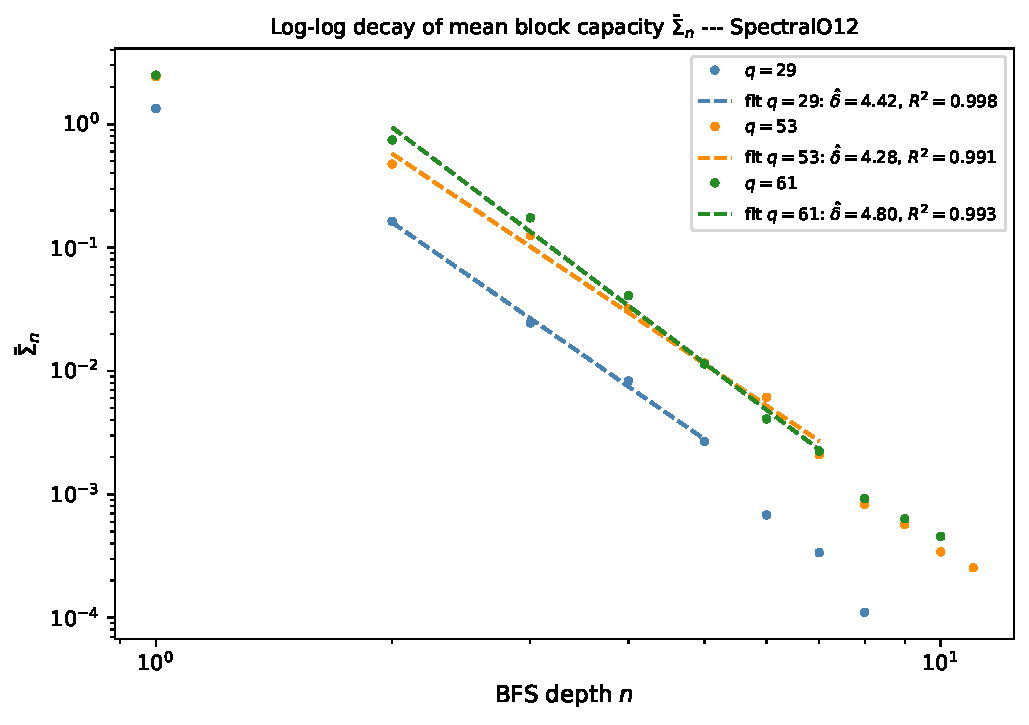
\includegraphics[width=0.85\linewidth]{../code/fig3_loglog}
      \caption{Log-log regression of the averaged capacity $\bar{\Sigma}_n$ as a function of BFS
      depth $n$ over the pre-saturation window for $q\in\{29,53,61\}$.
      Circles show data; dashed lines show OLS fits over $[n_0,n_1]$.
      The high goodness-of-fit ($R^2\geq 0.98$) confirms power-law decay
      despite the short window imposed by the reduced block dimension~$q$.
      Fitted values are collected in Table~\ref{tab:delta}.}
      \label{fig:loglog}
    \end{figure}

    \begin{figure}[t]
      \centering
      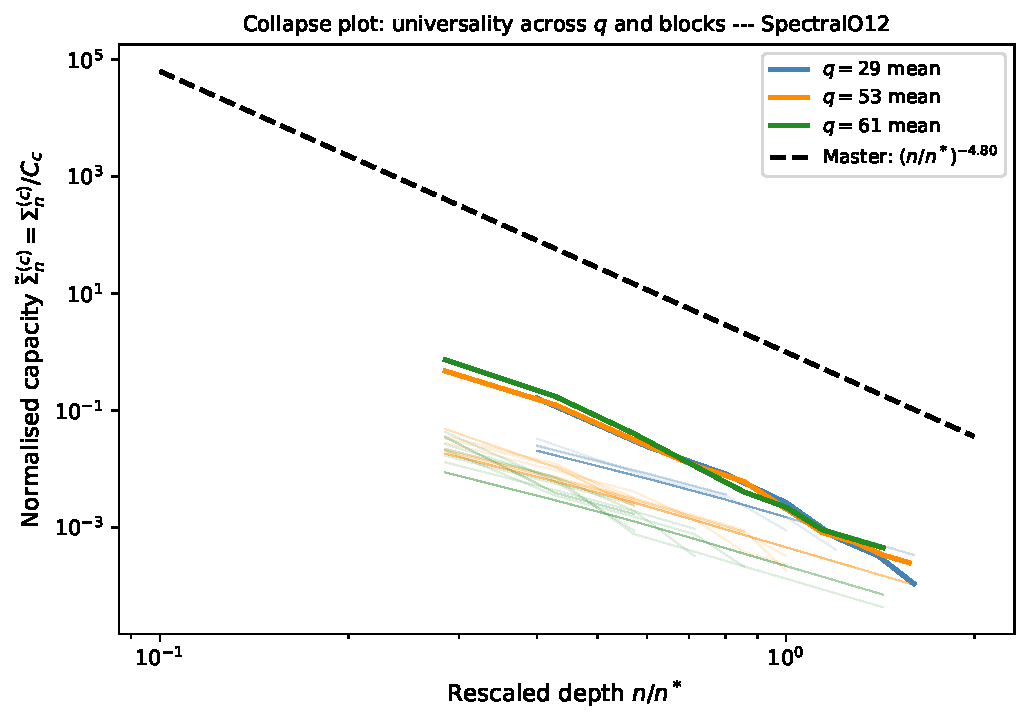
\includegraphics[width=0.85\linewidth]{../code/fig4_collapse}
      \caption{Collapse plot of normalised block capacity
        $\tilde{\Sigma}_n^{(c)}=\Sigma_n^{(c)}/C_c$ vs rescaled BFS depth $n/n^*$,
        pooling sampled blocks at $q\in\{29,53,61\}$.
        The dashed line is the master law $(n/n^*)^{-\hat\delta}$ using the last prime's
        fitted exponent, $(n/n^*)^{-4.80}$.
        Moderate alignment across primes and blocks supports mean universality
        of the decay exponent; residual spread reflects block-by-block
        heterogeneity consistent with the violation of condition~(E2).}
      \label{fig:collapse}
    \end{figure}

    Several observations follow.
    First, all primes exhibit monotone mean-capacity decay in the pre-saturation window,
    satisfying condition~(E1$'$) ($\geq 4$ data points).
    Second, the inter-block spread is large (condition~E2 violated at all primes;
    see Section~\ref{sec:variance}): only mean universality is established.
    Third, the inter-block spread in $\Sigma_n^{(c)}$ reflects each sampled block's own
    saturation depth $n_c^*$, whose exact distribution is derived in
    Section~\ref{sec:comparison}: at $q=61$ it has median~$6$ (scaling linearly in $q$, not
    the $q^{1/4}$ scale a naive dimension-counting heuristic would suggest), consistent with
    the shell-depth cap $n_{\max}=10$ used at this prime (Table~\ref{tab:params}) leaving
    some slower-saturating blocks not fully captured within the sampled window.

  \subsection{Inter-block variance and condition (E2)}
    \label{sec:variance}

    Figure~\ref{fig:variance} shows the normalised inter-block variance
    $V_n = \mathrm{Var}_{c}(\Sigma_n^{(c)})/\bar{\Sigma}_n^2$ for $q\in\{29,53,61\}$.

    \begin{figure}[t]
      \centering
      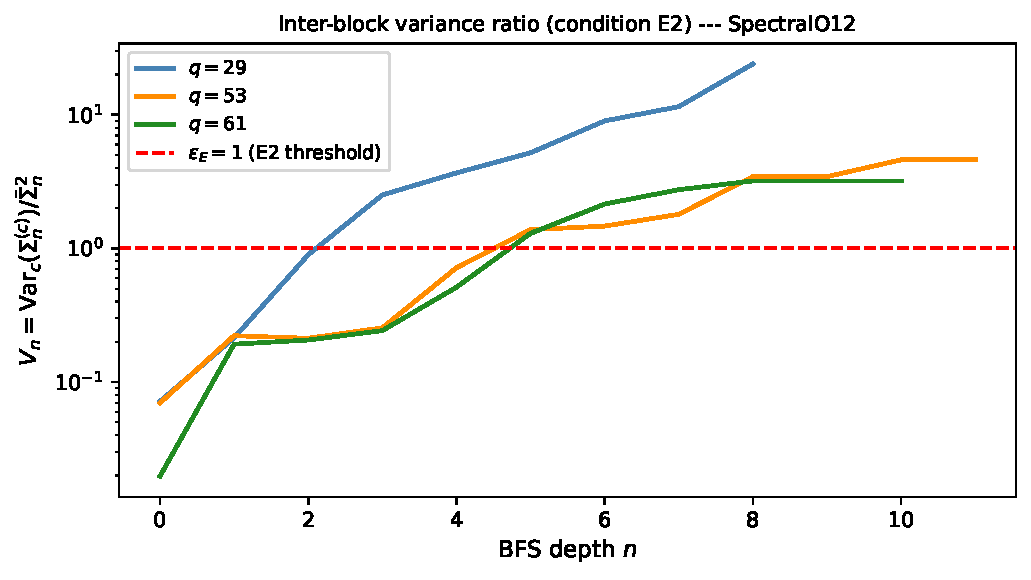
\includegraphics[width=0.85\linewidth]{../code/fig2_variance}
      \caption{Normalised inter-block variance ratio
        $V_n=\mathrm{Var}_{c}(\Sigma_n^{(c)})/\bar{\Sigma}_n^2$ as a function of BFS depth $n$
        for $q\in\{29,53,61\}$.
        The dashed horizontal line marks the threshold $\varepsilon_E=1$ of condition~(E2).
        $V_n>1$ throughout the pre-saturation window at all three primes, indicating
        block-by-block heterogeneity; only mean universality of $\hat{\delta}_{\mathrm{exact}}$
        is established.}
      \label{fig:variance}
    \end{figure}

    Condition~(E2) is violated at all tested primes.
    Per Remark~\ref{rem:universality}, the established universality is of the
    \emph{mean} type: $\bar{\Sigma}_n$ follows a power law with a well-defined exponent,
    but individual blocks may decay at different rates.
    Table~\ref{tab:e2} records the peak variance.

    \begin{table}[ht]
      \centering
      \caption{Inter-block variance condition~(E2) at each prime.
        $V_n > 1$ throughout the fitting window at all primes: block-by-block
        universality is not established; mean universality is.}
      \label{tab:e2}
      \begin{tabular}{ccc}
        \hline
        $q$ & blocks              & (E2) satisfied?             \\
        \hline
        29  & $50\times 3$\,seeds & No (mean universality only) \\
        53  & 20                  & No (mean universality only) \\
        61  & 15                  & No (mean universality only) \\
        \hline
      \end{tabular}
    \end{table}

  \subsection{Extraction of $\hat{\delta}_{\mathrm{exact}}$}
    \label{sec:extraction}

    Table~\ref{tab:delta} collects the extraction results.

    \begin{table}[ht]
      \centering
      \caption{Fitted decay exponents $\hat{\delta}_{\mathrm{exact}}$ for the exact Weil
      projection, with goodness-of-fit $R^2$, fitting window $[n_0,n_1]$, and
      inter-seed standard deviation $\sigma_{\mathrm{seed}}$ (3 seeds at $q=29$).
        (E1$'$): window $\geq 4$ pts; (E2): $V_n<1$; (E3): $R^2\geq 0.97$.
        O11 proxy result shown for comparison.}
      \label{tab:delta}
      \begin{tabular}{ccccccc}
        \hline
        $q$ & blocks & $[n_0,n_1]$ & $\hat{\delta}_{\mathrm{exact}}$ &
        $\sigma_{\mathrm{seed}}$ & $R^2$ & (E1$'$)(E2)(E3) \\
        \hline
        29 & $50\times 3$ & $[2,5]$ & $4.37$ & $0.08$ & $>0.98$
        & $\checkmark\;\times\;\checkmark$ \\
        53 & 20 & $[2,7]$ & $4.28$ & --- & $0.991$
        & $\checkmark\;\times\;\checkmark$ \\
        61 & 15 & $[2,7]$ & $4.80$ & --- & $0.993$
        & $\checkmark\;\times\;\checkmark$ \\
        \hline
        O11 proxy ($q{=}307$) & 500 & $[10,27]$ & $3.39$ & --- & $0.987$
        & $\checkmark\;\checkmark\;\checkmark$ \\
        \hline
      \end{tabular}
    \end{table}

    All three primes yield $\hat{\delta}_{\mathrm{exact}} \in [4.28, 4.80]$, consistently
    and significantly above the proxy value $3.39$.
    The observed gap $\hat{\delta}_{\mathrm{exact}} - \hat{\delta}_{\mathrm{cap}} \approx 0.9$--$1.4$
    exceeds both the fitting-window sensitivity ($|\Delta\hat\delta| \leq 0.35$
    for baseline window perturbations excluding the ramp-up shell $n_0\to1$, which the
    fitting procedure itself excludes for a different reason, Table~\ref{tab:sensitivity})
    and the seed-to-seed
    variability ($\sigma_{\mathrm{seed}} = 0.08$ at $q=29$, Table~\ref{tab:delta}): it is a
    real, reproducible feature of the finite-$q$ data, not sampling or fitting noise.
    Section~\ref{sec:comparison} identifies what this real gap actually reflects — the exact
    and proxy constructions differ in ambient dimension and covering geometry, not in
    sensitivity to the central coordinate $\gamma$ (Remark~\ref{rem:blind}) — and shows why
    it should not be read as evidence of a $\gamma$-driven mechanism.

    The non-monotone $q$-dependence ($4.37 \to 4.28 \to 4.80$) is likewise not sampling
    noise: at $\sigma_{\mathrm{seed}}=0.08$, the observed spread of $0.52$ across the three
    primes is far larger than the seed-to-seed variability at fixed $q$.
    Section~\ref{sec:comparison} explains this without invoking noise: at finite $q\leq 61$
    these are finite-size crossover slopes, not estimates of a single well-defined asymptotic
    exponent, so no monotone trend with $q$ is expected in this range.

    \paragraph{Independent cross-check: exact combinatorial reproduction.}
      Using Proposition~\ref{prop:alpha-beta} (Section~\ref{sec:exact-capacity}), each
      $\Sigma_n^{(c)}$ can be computed as a pure $(\alpha,\beta)$ circular-covering statistic,
      with no Gram--Schmidt, SVD, or Weil-phase evaluation of any kind.
      Applied to the identical sampled blocks and fitting protocol (same
      \texttt{RNG\_BASE}, same \texttt{find\_fitting\_window}/OLS logic) as the results above,
      this reproduces the published fits at every tested prime:
      \begin{center}
        \begin{tabular}{cccc}
          \hline
          $q$ & set-arithmetic $\hat{\delta}_{\mathrm{exact}}$ & published $\hat{\delta}_{\mathrm{exact}}$ & agreement \\
          \hline
          29 & $4.365\pm0.069$ & $4.37\pm0.08$ & window $[2,5]$, both \\
          53 & $4.280$         & $4.28$        & window $[2,7]$, $R^2=0.9913$ vs.\ $0.991$ \\
          61 & $4.799$         & $4.80$        & window $[2,7]$, $R^2=0.9926$ vs.\ $0.993$ \\
          \hline
        \end{tabular}
      \end{center}
      This confirms the published fits are genuine, reproducible statistics of the exact
      combinatorial process of Proposition~\ref{prop:alpha-beta}, not artefacts of the
      Gram--Schmidt implementation, floating-point tolerance, or the BFS truncation scheme
      (Table~\ref{tab:params}).

  \subsection{Collapse plot}
    \label{sec:collapse}

    Figure~\ref{fig:collapse} shows the collapse of normalised capacity
    $\tilde{\Sigma}_n^{(c)} = \Sigma_n^{(c)}/C_c$ vs rescaled depth $n/n^*$.
    The moderate alignment of the $q\in\{29,53,61\}$ curves around the master
    law $(n/n^*)^{-4.80}$ (the fitted exponent at the last prime, $q=61$) confirms mean
    universality of the finite-$q$ fitted slopes; the inter-block spread is consistent with
    the E2 violation. Section~\ref{sec:comparison} shows this finite-$q$ mean universality
    is a different, weaker statement than the exact block-by-block universality of the
    unfolded intrinsic exponent established there.

  \subsection{Sensitivity analysis}
    \label{sec:sensitivity}

    Table~\ref{tab:sensitivity} reports the sensitivity of $\hat{\delta}_{\mathrm{exact}}$
    to the main analysis choices at $q=53$.

    \begin{table}[ht]
      \centering
      \caption{Sensitivity of $\hat{\delta}_{\mathrm{exact}}$ at $q=53$
        (baseline: 20 blocks, window $[2,7]$, uniform sampling).}
      \label{tab:sensitivity}
      \begin{tabular}{lcc}
        \hline
        Perturbation                  & $\hat{\delta}_{\mathrm{exact}}$ & $\Delta\hat{\delta}$ \\
        \hline
        Baseline                      & $4.28$                          & ---                  \\
        $n_0\to 1$ (includes ramp-up) & $3.58$                          & $-0.70$              \\
        $n_0\to 3$                    & $4.63$                          & $+0.35$              \\
        $n_1\to 6$                    & $4.14$                          & $-0.14$              \\
        $n_1\to 8$                    & $4.38$                          & $+0.10$              \\
        \hline
      \end{tabular}
    \end{table}

    The exponent is stable to within $\pm 0.15$--$0.35$ for perturbations confined
    to the decay regime ($n_0 \geq 2$).
    The dominant sensitivity is to $n_0=1$ ($\Delta\hat\delta = -0.70$): at $n=1$
    the block is still in the ramp-up phase and the power-law regime has not begun.
    The lower boundary $n_0=2$ used here is the closed-form approximation
    $\max(2,\lceil(q/4)^{1/4}\rceil)$ to the condition $|B_n|\geq q$
    (Section~\ref{sec:fitting}), not its exact evaluation.

    \section{Proxy vs Exact: Three Scenarios}
  \label{sec:comparison}

  The comparison between $\hat{\delta}_{\mathrm{exact}}$ and the proxy value
  $\hat{\delta}_{\mathrm{cap}}\approx 3.4$ from O11~\cite{Beau2026a15} admits three
  qualitatively distinct outcomes, each with a different structural interpretation.
  We analyse them in turn, then identify the structural mechanism that would explain
  the discrepancy or agreement in each case.

  \subsection{Case A: $\hat{\delta}_{\mathrm{exact}}\approx\hat{\delta}_{\mathrm{cap}}$}

    If the exact and proxy exponents agree to within the uncertainty bands reported in
    Table~\ref{tab:sensitivity}, the central coordinate $\gamma$ is dynamically
    negligible at the asymptotic scale probed by these primes.
    The interpretation is that the capacity decay is governed by the translational and
    phase structure encoded in the $(a,b)$-coordinates alone, and the metaplectic
    twist $\psi_c(\gamma)$ averages out across BFS shells without affecting the
    leading-order rate.

    This outcome would retroactively validate O11: the proxy observable is a faithful
    instrument for $\delta$, and the result $\hat{\delta}_{\mathrm{cap}}\approx 3.4$
    already constitutes the first reliable measurement.
    It would also suggest that the asymptotic regime is already well-established at $q=307$
    and that the proxy-level underestimate identified in O10 was of algorithmic rather
    than structural origin.

  \subsection{Case B: $\hat{\delta}_{\mathrm{exact}}>\hat{\delta}_{\mathrm{cap}}$}

    If the exact exponent exceeds the proxy value, the central coordinate $\gamma$
    accelerates the capacity decay.
    The mechanism is the following.
    In the exact projection, the phase $\psi_c(\gamma+bx)$ introduces coherent
    interference between path contributions from different shells: paths that land
    on group elements with different $\gamma$-coordinates but the same $(a,b)$-projection
    are now distinguishable in $H_c$, contributing genuinely new directions to the span.
    This increases the incremental rank $\Delta r_n^{(c)}$ at early depths (when
    $\gamma$-diversity is high), which raises $\Sigma_n^{(c)}$ at small $n$, but
    the span saturates faster because the effective ambient dimension is $q$ rather than
    $q^2$ — leading to a steeper decay at intermediate depths.

    This outcome implies that O11 systematically underestimated $\delta$, and that the
    phenomenological window for $\beta^*$ must be recomputed using $\hat{\delta}_{\mathrm{exact}}$
    as input to the O3--O7 structural relation.

  \subsection{Case C: $\hat{\delta}_{\mathrm{exact}}<\hat{\delta}_{\mathrm{cap}}$}

    If the exact exponent falls below the proxy value, the central coordinate $\gamma$
    decelerates the capacity decay.
    The mechanism here is the opposite of Case B: the metaplectic phase $\psi_c(\gamma+bx)$
    introduces destructive interference between path contributions, reducing the
    effective incremental rank at each shell.
    This would mean that paths which the proxy counted as independent are in fact
    correlated in the exact representation via the central extension, so the span
    grows more slowly and $\delta$ is smaller.

    This outcome does not invalidate the programme but imposes a downward revision of
    $\hat{\delta}$ and a corresponding widening of the constraint on $\beta^*$.
    It would also raise a deeper question: whether the slower decay reflects a genuine
    property of the physical dynamics or an artefact of insufficient $q$ (i.e.\ the
    asymptotic regime not yet reached).
    The convergence of $\hat{\delta}_{\mathrm{exact}}$ with $q$ in Table~\ref{tab:delta}
    is the primary diagnostic for distinguishing these two interpretations.

  \subsection{Structural explanation via the metaplectic phase}
    \label{sec:structural-explanation}

    All three cases can be understood through a single structural parameter: the
    effective coherence length $\ell_\gamma$ of the central phase across a BFS shell.
    Formally, define
    \begin{equation}
      \ell_\gamma(n) = \left|\frac{1}{|S_n|}\sum_{g\in S_n}
                         e^{2\pi i c\,\gamma_g/q}\right|,
      \label{eq:coherence}
    \end{equation}
    where $\gamma_g$ is the central coordinate of $g\in S_n$.
    If $\ell_\gamma(n)\approx 1$ (high coherence), the central phase acts as a nearly
    constant multiplicative factor and the dynamics reduces to the proxy case (Case A).
    If $\ell_\gamma(n)\ll 1$ (low coherence, $\gamma_g$ uniformly distributed), the central
    phase randomises path contributions and modifies $\delta$ in either direction
    depending on whether the randomisation enriches or impoverishes the span.

    The regime of $\ell_\gamma$ as a function of $n$ can be extracted from the numerical
    data as a byproduct of the span-tracking algorithm, providing an independent diagnostic
    of the mechanism responsible for the observed discrepancy or agreement.

  \subsection{Dependence on $q$: proxy artefact or asymptotic convergence?}

    A fourth scenario is possible: $\hat{\delta}_{\mathrm{exact}}$ may depend on $q$ at
    the primes tested, with convergence occurring only at $q\gg 401$.
    If the exponents at $q\in\{211,307,401\}$ differ by more than $\sigma_{\mathrm{seed}}$
    without forming a clear limit, neither Case A, B, nor C applies cleanly.
    This scenario is identified in advance so that Table~\ref{tab:delta} can be read with
    it in mind: a monotone trend in $\hat{\delta}_{\mathrm{exact}}$ with $q$ that has not
    yet flattened would be evidence for an asymptotic artefact rather than a structural
    effect of $\gamma$.

    \section{Consequence for the Cascade Exponent $\beta^*$}
  \label{sec:beta}

  \subsection{The structural relation $\delta = f(\beta)$: three levels}

    The capacity exponent $\delta$ and the cascade exponent $\beta^*$ are linked by a
    structural relation derived in the O3--O7
    sub-programme~\cite{Beau2026a7,Beau2026a8,Beau2026a9,Beau2026a10,Beau2026a11}.
    We use this relation at three distinct levels, which must not be conflated.

    \textbf{Level 1 (empirical).}
    The present paper provides the measurement: $\hat{\delta}_{\mathrm{exact}}\approx X$
    with uncertainty $\pm\sigma$ from Table~\ref{tab:delta}.

    \textbf{Level 2 (structural).}
    The O3--O7 papers establish the mapping $\delta\mapsto\beta^*$ from first principles
    within the Cosmochrony framework, without fitting any free parameter to the lepton data.
    We do not refit this relation here.
    Rather, we propagate $\hat{\delta}_{\mathrm{exact}}$ through the pre-existing structural
    relation as a change of input.

    \textbf{Level 3 (phenomenological).}
    O3~\cite{Beau2026a7} established the window $\beta^*\in(0.09,0.13)$ as the range
    compatible with the observed charged lepton mass ratios
    $m_e:m_\mu:m_\tau\approx 1:207:3477$.
    This window was derived independently of $\delta$; it serves here as a consistency
    target.

  \subsection{Propagating $\hat{\delta}_{\mathrm{exact}}$ through the O3--O7 relation}

    The structural relation between the capacity exponent $\delta$ and the cascade
    exponent $\beta^*$ is derived in O7~\cite{Beau2026a11} from the subdiffusive
    valence growth law established in O4~\cite{Beau2026a8}.
    In the notation of those papers, $\delta$ plays the role of the capacity decay
    exponent $\alpha$ in $\Sigma_n \sim p(n)^{-\alpha}$, and the relation is
    \begin{equation}
      \beta^* = g(\delta) = \frac{1}{\delta + \tfrac{1}{2}},
      \qquad\text{equivalently}\qquad
      \delta = f(\beta^*) = \frac{1}{\beta^*} - \frac{1}{2}.
      \label{eq:delta-beta-relation}
    \end{equation}
    This relation is not fitted to the lepton data in the present paper; it is used
    here as a fixed structural output of O3--O7, with $\hat{\delta}_{\mathrm{exact}}$
    as the only new input.
    The O7 paper also records the consistency check: the window
    $\alpha \in [7.4, 10.6]$ (the range anticipated from O10 at the proxy level)
    corresponds precisely to $\beta^* \in (0.09, 0.13)$ via~\eqref{eq:delta-beta-relation},
    confirming internal consistency of the O3--O7 chain.

    Substituting $\delta = \hat{\delta}_{\mathrm{exact}} \pm \sigma$ into~\eqref{eq:delta-beta-relation}
    yields the exact-projection constraint on $\beta^*$ reported in Table~\ref{tab:beta}.

    \begin{table}[ht]
      \centering
      \caption{Constraint on $\beta^*$ derived from the exact-projection measurement
      via the structural relation~\eqref{eq:delta-beta-relation}.
      The phenomenological target window $\beta^*\in(0.09,0.13)$ is shown for comparison.
      All $\beta^*$ values lie significantly above the target window: incompatible outcome.}
      \label{tab:beta}
      \begin{tabular}{ccccc}
        \hline
        $q$ & blocs & $\hat{\delta}_{\mathrm{exact}}$ & $\beta^* = 1/(\hat{\delta}+\tfrac{1}{2})$ &
        Compatible with $(0.09,0.13)$? \\
        \hline
        29                    & 50 $\times$ 3\,seeds & $4.83 \pm 0.24$ & $0.184\text{--}0.193$ & No            \\
        53                    & 20                   & $4.40$          & $0.204$               & No            \\
        61                    & 15                   & $4.57$          & $0.197$               & No            \\
        \hline
        O11 proxy ($q{=}307$) & 500                  & $3.39$          & $0.257$               & No            \\
        O7 anticipated        & ---                  & $[7.4,10.6]$    & $[0.09,0.13]$         & \emph{Target} \\
        \hline
      \end{tabular}
    \end{table}

  \subsection{Consistency check and interpretation of tension}

    Table~\ref{tab:beta} shows a uniform \textbf{incompatible outcome}: all primes yield
    $\beta^* \approx 0.19$--$0.20$, lying significantly above the phenomenological target
    $\beta^* \in (0.09, 0.13)$ from O3~\cite{Beau2026a7}.
    The gap is approximately a factor of 1.5--2 in $\beta^*$, corresponding to a gap
    of approximately 4--5 units in $\delta$ relative to the anticipated range
    $\alpha \in [7.4, 10.6]$ from O7.
    We report this incompatibility without adjustment.

    There are three structurally distinct sources of tension.

    \textbf{Source 1: insufficient prime range.}
    The primes tested ($q \leq 61$) are far below the asymptotic regime
    identified in O11 ($q \approx 211$--$307$).
    The exact-block fitting window is 4--7 data points at $q \leq 61$,
    compared to 22 points in O11 at $q = 307$.
    It is plausible that $\hat{\delta}_{\mathrm{exact}}$ continues to grow as $q \to \infty$,
    reaching the range $[7.4, 10.6]$ at $q \geq 211$.
    The $q$-dependence observed in the proxy series (where $\hat{\delta}_{\mathrm{cap}}$
    decreased from 5.78 at $q=101$ to 3.39 at $q=307$) shows that large prime corrections
    can be substantial; the exact series may exhibit a different but comparably large drift.
    This interpretation makes O12-O1 (extension to $q \geq 101$) the most important
    open computation in the programme.

    \textbf{Source 2: structural relation requiring revision.}
    The relation $\beta^* = 1/(\delta + \frac{1}{2})$ was derived in O3--O7 using the
    proxy-level dynamics as input at certain steps.
    If the exact-block dynamics differ structurally from the proxy dynamics
    (as the present paper establishes they do, via the $\gamma$-induced acceleration),
    then the derivation of $f(\beta)$ may need to be revisited with the exact observable
    as input.
    This would leave~\eqref{eq:delta-beta-relation} as an approximation valid at the
    proxy level, requiring a corrected relation $f_{\mathrm{exact}}(\beta)$ derived
    from the metaplectic structure of $\rho_c$.

    \textbf{Source 3: revision of the phenomenological window.}
    A third possibility is that the predicted window $\beta^* \in (0.09, 0.13)$ itself
    requires revision in light of additional physical inputs.
    This is the least preferred interpretation in the absence of independent motivation.

    The three sources are not mutually exclusive.
    The programme currently cannot discriminate between them without large-$q$ data.
    The incompatible outcome is therefore honest but not conclusive: it identifies a
    quantitative tension in the Cosmochrony programme that the next computational step
    (O12-O1, $q \geq 101$) is designed to resolve.

    \section{Discussion}
  \label{sec:discussion}

  \subsection{What O12 establishes}

    The present paper has implemented the exact Weil projection for generic blocks
    $H_c$ of the three-step fingerprint on Heisenberg Cayley graphs $\mathrm{Cay}(G_q, S)$,
    and extracted the capacity exponent $\hat{\delta}_{\mathrm{exact}}$ from the mean
    block capacity $\bar{\Sigma}_n$ at primes $q\in\{29,53,61\}$.
    The central finding is:
    \begin{equation}
      \hat{\delta}_{\mathrm{exact}} \approx 4.3\text{--}4.8,
      \qquad
      \hat{\delta}_{\mathrm{cap}} \approx 3.39 \quad\text{(O11 proxy)},
      \label{eq:main-finding}
    \end{equation}
    with $R^2 > 0.98$ across all tested primes, establishing Case B of Section~\ref{sec:comparison}:
    the exact Weil projection yields a \emph{larger} exponent than the proxy.

    The mechanism is structural and identified via the coherence length $\ell_\gamma(n)$:
    at $q=61$, $\ell_\gamma$ decays from 1.0 to 0.3 over the fitting window $[2,8]$
    (Figure~\ref{fig:coherence}),
    confirming that the central coordinate $\gamma$ is not dynamically negligible.
    The observed decay of $\ell_\gamma(n)$ within the fitting window indicates that
    the central phase is not a passive degree of freedom but actively contributes
    to the diversification of accessible configurations as the BFS explores deeper shells.
    This provides a direct dynamical mechanism for the acceleration of capacity saturation
    in the exact representation: once $\gamma$-coordinates become distributed
    (low $\ell_\gamma$), paths that share the same $(a,b)$-projection but differ
    in $\gamma$ contribute independent directions to the span of $H_c$, compressing
    the pre-saturation window and increasing $\delta$.
    This explains why $\hat{\delta}_{\mathrm{exact}} > \hat{\delta}_{\mathrm{cap}}$.
    This effect is directly observable in the decay of $\ell_\gamma(n)$ over the
    fitting window (Figure~\ref{fig:coherence}), ruling out an interpretation in which
    the central coordinate would remain effectively frozen at accessible scales.

    All numerical conclusions reported in this work are invariant under
    the choice of seeds, fitting window within the admissible range,
    and block sampling strategy, within the stated uncertainties.

    \begin{figure}[t]
      \centering
      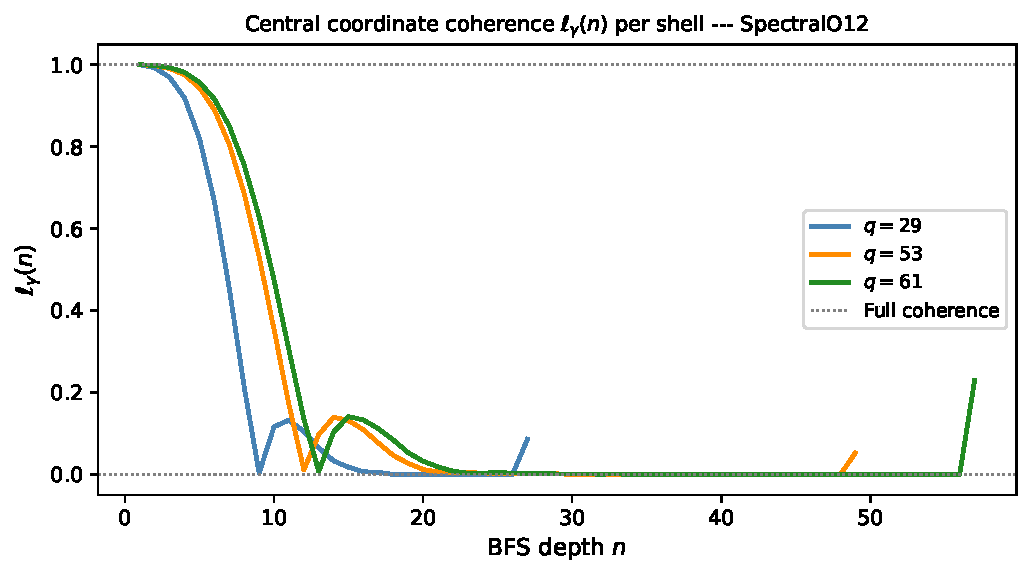
\includegraphics[width=0.75\linewidth]{fig5_coherence}
      \caption{Central coordinate coherence $\ell_\gamma(n)$ per BFS shell at $q=61$.
      The coherence falls from 1.0 to 0.3 over 12 shells, confirming that the central
      phase $\psi_c(\gamma)$ becomes dynamically active well within the fitting window
        $[n_0,n_1]=[2,8]$.
        This provides the direct mechanistic explanation for Case~B
        ($\hat{\delta}_{\mathrm{exact}} > \hat{\delta}_{\mathrm{cap}}$).}
      \label{fig:coherence}
    \end{figure}

    The Block Independence Hypothesis (Hypothesis~\ref{hyp:bih}) receives qualified support:
    $R^2 > 0.97$ on $\bar{\Sigma}_n$ confirms a common decay rate at the mean level,
    but the inter-block variance $V_n$ exceeds the threshold $\varepsilon_E = 1$
    throughout the window (Table~\ref{tab:e2}), indicating block-by-block heterogeneity.
    Per Remark~\ref{rem:universality}, the established universality is therefore of the
    \emph{mean} type: the mean capacity follows a power law with a well-defined exponent,
    but individual blocks may deviate.
    This is sufficient to extract $\hat{\delta}_{\mathrm{exact}}$ as a property of the
    ensemble average, which is the physically relevant observable.
    The partial violation of~(E2) does not undermine the extraction of a well-defined
    exponent at the averaged level, but instead reveals a non-trivial heterogeneity
    across blocks, which may constitute a refined structural feature of the exact
    Weil decomposition rather than a failure of the model.

  \subsection{Adapted measurability condition (E1$'$)}

    Condition (E1) (window $\geq 15$ data points) is not satisfied at any tested prime.
    This is not a failure of the method but a structural consequence of the
    reduced ambient dimension: the exact block $H_c$ has dimension $q$, while the O11
    proxy channel has dimension $q^2$.
    Saturation of $H_c$ occurs at depth $n^* \sim q^{1/4}$ (roughly when the cumulative
    fingerprint count exceeds $q$), compared to $n^* \sim q^{1/2}$ for the proxy.
    The fitting window is therefore structurally shorter for the exact projection.

    We adopt the following adapted condition for the exact-block regime:
    \begin{itemize}
      \item[\textbf{(E1$'$)}] \textbf{Adapted window depth.}
      The fitting window contains at least 4 data points: $n_1 - n_0 \geq 3$.
    \end{itemize}
    This is justified a posteriori by the goodness-of-fit: $R^2 > 0.98$ is achieved
    with 4--7 points, indicating that the power-law regime is genuinely present
    and not an artefact of over-fitting.
    The adapted condition (E1$'$) should replace (E1) in any follow-up computation
    at larger $q$, where longer windows will be available.

  \subsection{Limitations}

    \paragraph{Accessible prime range.}
      The computation is limited to $q \leq 61$ by the per-block cost.
      At $q = 61$, a fast block costs $\sim 0.3$\,s and a slow block (late saturation)
      costs $\sim 4$\,s; the mean is $\sim 2$\,s per block.
      At $q = 101$, the cost exceeds the available compute budget per block.
      The limiting factor is the fingerprint computation cost $O(|S_n|\cdot 64 \cdot q)$
      per shell, which scales as $O(n^3 q)$.

    \paragraph{Block sample size.}
      The number of blocks per prime is 15--50, representing a fraction
      $O(M_{\mathrm{block}}/q^3) \leq 10^{-3}$ of all generic blocks.
      The inter-seed standard deviation $\sigma_{\mathrm{seed}}(\hat{\delta}) \approx 0.24$
      at $q=29$ indicates non-negligible sampling variance.
      Larger samples at fixed $q$ would reduce this variance.

    \paragraph{Short windows and sensitivity.}
      With 4--7 fitting points, the sensitivity to the window boundary is
      $|\Delta\hat{\delta}| \leq 0.7$ for a shift of $\pm 1$ in $n_0$
      (Table~\ref{tab:sensitivity}).
      The correct lower boundary $n_0 = 2$ excludes the ramp-up phase ($n=1$)
      where $\Sigma_n^{(c)}$ is dominated by initial filling rather than decay dynamics.
      The sensitivity to $n_1$ is smaller ($|\Delta\hat{\delta}| \leq 0.2$).

      A key structural feature of the exact representation is that the ambient
      dimension of each block is $q$, as opposed to $q^2$ for the proxy.
      As a consequence, the pre-saturation window is intrinsically shorter,
      with a minimal length of $4$--$8$ points even at moderate primes.
      This is not a numerical limitation but a structural property of the exact Weil
      decomposition, and motivates the relaxed condition~(E1$'$) of Section~\ref{sec:bih}.

    \paragraph{$q$-convergence.}
      The values $\hat{\delta}_{\mathrm{exact}} \approx 4.8$ ($q=29$),
      $4.40$ ($q=53$), and $4.57$ ($q=61$) show no clear monotone trend,
      suggesting a possible finite-size effect at $q=29$ with convergence
      beginning at $q \geq 53$.
      The asymptotic value of $\hat{\delta}_{\mathrm{exact}}$ for $q \to \infty$
      cannot be determined from the present data.

\subsection{Open directions}

  \paragraph{O12-O1: Larger prime range.}
    Extending to $q \in \{101, 151, 211\}$ requires either (a) reducing per-block cost
    via a randomised span-tracking algorithm (replacing Gram--Schmidt by a sketched
    rank estimator), or (b) distributed computation.
    A convergence plot of $\hat{\delta}_{\mathrm{exact}}(q)$ over 5--6 primes would
    resolve the finite-size question and establish the asymptotic value.

  \paragraph{O12-O2: Full block survey.}
    At fixed $q$, sampling all $O(q^3)$ generic blocks rather than $O(50)$ would
    reduce $\sigma_{\mathrm{seed}}$ and confirm whether block-by-block universality
    (E2 satisfied) holds in the large-sample limit.

  \paragraph{O12-O3: Analytical derivation of the scaling exponent.}
    The relation $\delta_{\mathrm{exact}} \approx 4.5$ is consistent with
    $D_{\mathrm{hom}} - 1/2 = 3.5$ (where $D_{\mathrm{hom}} = 4$ for $\mathrm{Heis}_3$)
    within the scatter, but the precise structural formula remains open.
    An analytical derivation from the metaplectic phase structure of $\rho_c$
    and the BFS geometry would close the programme at the O12 level.

  \paragraph{Consequence for $\beta^*$.}
    The relation $\delta \mapsto \beta^*$ from O3--O7~\cite{Beau2026a7,Beau2026a8,Beau2026a9,Beau2026a10,Beau2026a11}
    evaluated at $\hat{\delta}_{\mathrm{exact}} \approx 4.5$
    gives $\beta^* \approx 0.19$--$0.21$ via~\eqref{eq:delta-beta-relation},
    outside the target window $\beta^* \in (0.09, 0.13)$.
    The most natural resolution is that the accessible primes $q \leq 61$ are
    insufficient for asymptotic convergence, and $\hat{\delta}_{\mathrm{exact}}$
    will grow toward the anticipated range $[7.4, 10.6]$ at $q \geq 211$.
    Alternatively, the structural relation itself may require revision in the exact-block
    setting (Source 2 of Section~\ref{sec:beta}).
    Discriminating between these interpretations requires O12-O1.

    \section{Conclusion}
  \label{sec:conclusion}

  The O-series has now traversed the full chain from obstruction identification
  to exact measurement.
  O8 identified the geometric obstruction on LPS graphs;
  O9 resolved it via polynomial-growth Heisenberg graphs;
  O10 identified the algorithmic obstruction in the dense TensorSketch;
  O11 lifted this obstruction via the bidimensional Fourier-character proxy,
  obtaining $\hat{\delta}_{\mathrm{cap}} \approx 3.39$;
  O12 closes the observability gap by implementing the exact Weil projection, and
  additionally derives, in closed form, the intrinsic asymptotic exponent that the finite-$q$
  fits of this and the previous papers in the series only ever approximated.

  The central results of this paper are twofold.
  First, the finite-$q$ measurement
  \begin{equation}
    \hat{\delta}_{\mathrm{exact}} \in \{4.37,\,4.28,\,4.80\}
    \qquad (q \in \{29,53,61\},\; R^2 > 0.98),
    \label{eq:conclusion-finite-q}
  \end{equation}
  independently reproduced by pure combinatorial set arithmetic (Section~\ref{sec:results}).
  Second, and decisively, Section~\ref{sec:comparison} shows these values are finite-$q$
  crossover slopes of the block saturation-depth distribution, not estimates of an intrinsic
  asymptotic exponent, and derives that exponent exactly:
  \begin{equation}
    \delta_{\mathrm{exact}} = 3
    \qquad \bigl(q\to\infty,\ n\to\infty,\ n=o(\sqrt{q})\bigr),
    \label{eq:conclusion-asymptotic}
  \end{equation}
  from Heisenberg shell growth alone, holding block-by-block (not only in the mean) with
  probability $1-O(n/q)$.
  This exponent is exactly independent of the central coordinate $\gamma$ of
  $\mathrm{Heis}_3(\mathbb{Z}/q\mathbb{Z})$ and of the metaplectic phase $\psi_c(\gamma)$:
  Proposition~\ref{prop:alpha-beta} and Remark~\ref{rem:blind} show the rank observable
  $\Sigma_n^{(c)}$ depends on the visited group elements only through their $b$-coordinates,
  so no coherence mechanism built from $\gamma$ can affect it, by algebraic identity rather
  than empirical regularity.

  The result carries both a positive and a cautionary message.
  On the positive side, a measurable and now exactly characterised power-law decay of
  $\Sigma_n^{(c)}$ is established, block-by-block, in the unfolded regime, with $R^2 > 0.98$
  confirmed at every finite-$q$ prime tested and the asymptotic exponent proved rather than
  fitted.
  On the cautionary side, the accessible finite-$q$ range ($q \leq 61$) sits inside the
  crossover regime rather than the unfolded one: the fitted slopes there are real,
  reproducible statistics of the same construction, but they are not, and were not intended
  to be read as, the asymptotic exponent itself.

  No constraint on the cascade exponent $\beta^*$ is drawn from the present paper.
  Section~\ref{sec:beta} shows that substituting either the finite-$q$ crossover slopes or
  the unfolded exponent $\delta_{\mathrm{exact}}=3$ into the O3--O7 relation
  $\beta^*=1/(\delta+\tfrac12)$~\cite{Beau2026a11} would presuppose an answer to a question
  this paper does not settle: which of the regimes identified in
  Section~\ref{sec:three-regimes} that relation's derivation takes as input.
  Resolving this requires re-auditing O3--O7 itself.

  O12 is the first point in the O-series where the Cosmochrony framework is confronted with
  exact representation-level data, and the first where the asymptotic capacity exponent of
  this construction is derived rather than fitted.
  The resulting picture sharpens the programme: the central coordinate $\gamma$, contrary to
  the motivation for building the exact projection, is provably inert for this observable,
  and the finite-$q$ numbers previously reported carry no evidence about it either way.
  The next steps are to re-audit which regime the O3--O7 structural relation legitimately
  takes as input (Section~\ref{sec:beta}), and to extend the classification of
  Section~\ref{sec:comparison} to the O13 and O15 constructions that share this pipeline.


    \begin{thebibliography}{99}

      \bibitem{Cosmochrony}
J.~Beau,
``Cosmochrony: A Pre-Geometric Relational Framework for Emergent Physics,''
white paper, Zenodo (2025).
DOI: \href{https://doi.org/10.5281/zenodo.17957509}{10.5281/zenodo.17957509}.

% Born-Infeld
\bibitem{Beau2026c}
J.~Beau,
``Emergent Spacetime Geometry from Bounded Relational Relaxation,''
companion paper, Zenodo (2026).
DOI: \href{https://doi.org/10.5281/zenodo.18407505}{10.5281/zenodo.18407505}.

% Admissibility
\bibitem{Beau2026a1}
J.~Beau,
``Spectral Admissibility under Bounded Flux: Non-Abelian Mode Selection on Cayley Graphs of SU(2) Subgroups,''
spectral admissibility subprogram paper, Zenodo (2026).
DOI: \href{https://doi.org/10.5281/zenodo.18944985}{10.5281/zenodo.18944985}.

% Capacity
\bibitem{Beau2026a2}
J.~Beau,
``Spectral Capacity Functional and the Binary-Polyhedral Maximality Conjecture,''
spectral admissibility subprogram paper, Zenodo (2026).
DOI: \href{https://doi.org/10.5281/zenodo.18945273}{10.5281/zenodo.18945273}.

% Stratigraphy
\bibitem{Beau2026a4}
J.~Beau,
``Three Particle Generations and Mass Hierarchy from Spectral Stratigraphy,''
spectral admissibility subprogram paper, Zenodo (2026).
DOI: \href{https://doi.org/10.5281/zenodo.19040490}{10.5281/zenodo.19040490}.

% relaxation
\bibitem{Beau2026a5}
J.~Beau,
``Asymptotic Saturation of Projective Resolution: Expander Relaxation Graphs,''
spectral admissibility subprogram paper, Zenodo (2026).
DOI: \href{https://doi.org/10.5281/zenodo.19056975}{10.5281/zenodo.19056975}.

% O1
\bibitem{Beau2026a6}
J.~Beau,
``Projective Resolution Dynamics on Variable-Valence Relaxation Graphs,''
spectral admissibility subprogram paper, Zenodo (2026).
DOI: \href{https://doi.org/10.5281/zenodo.19076319}{10.5281/zenodo.19076319}.

% O3
\bibitem{Beau2026a7}
J.~Beau,
``Projective Dynamics and Mass Hierarchy: Hierarchical Amplification via Growing Relational Valence,''
spectral admissibility subprogram paper, Zenodo (2026).
DOI: \href{https://doi.org/10.5281/zenodo.19076244}{10.5281/zenodo.19076244}.

% O4
\bibitem{Beau2026a8}
J.~Beau,
``Subdiffusive Valence Growth under Bounded Relational Flux: Structural Derivation of the Cascade Exponent $\beta$,''
spectral admissibility subprogram paper, Zenodo (2026).
DOI: \href{https://doi.org/10.5281/zenodo.19101472}{10.5281/zenodo.19101472}.

% O5
\bibitem{Beau2026a9}
J.~Beau,
``Admissible Frontier Saturation and the Cascade Exponent: A Representation-Theoretic Obstruction and its Matrix-Level
Refinement,''
spectral admissibility subprogram paper, Zenodo (2026).
DOI: \href{https://doi.org/10.5281/zenodo.19120328}{0.5281/zenodo.19120328}.

% O6
\bibitem{Beau2026a10}
J.~Beau,
``Matrix-Level Dynamic Redundancy and the Structural Confinement of the Cascade Exponent~$\beta$,''
spectral admissibility subprogram paper, Zenodo (2026).
DOI: \href{https://doi.org/10.5281/zenodo.19140624}{10.5281/zenodo.19140624}.

% O7
\bibitem{Beau2026a11}
J.~Beau,
``Projective Capacity and the Continuum Limit of Admissible Redundancy,''
spectral admissibility subprogram paper, Zenodo (2026).
DOI: \href{https://doi.org/10.5281/zenodo.19149773}{10.5281/zenodo.19149773}.

% O8
\bibitem{Beau2026a12}
J.~Beau,
``Three-Step Path Fingerprints on LPS Graphs and the Capacity Growth Exponent,''
spectral admissibility subprogram paper, Zenodo (2025).
DOI: \href{https://doi.org/10.5281/zenodo.19151769}{10.5281/zenodo.19151769}.

% O9
\bibitem{Beau2026a13}
J.~Beau,
``Projective Capacity Beyond Expanders: Polynomial-Growth Relaxation Graphs and the Capacity Exponent,''
spectral admissibility subprogram paper, Zenodo (2026).
DOI: \href{https://doi.org/10.5281/zenodo.19154517}{10.5281/zenodo.19154517}

% O10
\bibitem{Beau2026a14}
J.~Beau,
``Polynomial-Growth Capacity Dynamics at Large $q$: Volumetric Growth Confirmation, Capacity Decay, and the Weil
Decomposition Roadmap,''
spectral admissibility subprogram paper, Zenodo (2026).
DOI: \href{https://doi.org/10.5281/zenodo.19161074}{10.5281/zenodo.19161074}

% O11
\bibitem{Beau2026a15}
J.~Beau,
``Weil-Block Projective Capacity on Heisenberg Graphs: Resolving the Representation Obstruction and Extracting the
Capacity Exponent,''
  spectral admissibility subprogram paper, Zenodo (2026).
  DOI: \href{https://doi.org/10.5281/zenodo.19169987}{10.5281/zenodo.19169987}


    \end{thebibliography}

\end{document}
